\documentclass[conference]{IEEEtran}
\usepackage{cite}
\usepackage{amsmath,amssymb,amsfonts}
\usepackage{algorithmic}
\usepackage{graphicx}
\usepackage{textcomp}
\usepackage{xcolor}
\usepackage{tikz}
\usetikzlibrary{shapes, arrows}
\graphicspath{{./images/}}

\def\BibTeX{{\rm B\kern-.05em{\sc i\kern-.025em b}\kern-.08em
    T\kern-.1667em\lower.7ex\hbox{E}\kern-.125emX}} 
% Preamble for page numbering

\begin{document}

\title{On Wireless Audio: A Brief Literature Review}

\author{\IEEEauthorblockN{Diego Cruz}
    \IEEEauthorblockA{\textit{Dept. of Computer Engineering} \\
        \textit{San Jose State University}\\
        San Jose, United States \\
        diego.cruz@sjsu.edu}
    \and
    \IEEEauthorblockN{Shiv Shankar Yadav}
    \IEEEauthorblockA{\textit{Dept. of Computer Engineering} \\
        \textit{San Jose State University}\\
        San Jose, United States \\
        shivshankar.yadav@sjsu.edu}
    \and
    \IEEEauthorblockN{Mahima Agumbe Suresh}
    \IEEEauthorblockA{\textit{Dept. of Computer Engineering} \\
        \textit{San Jose State University}\\
        San Jose, United States \\
        mahima.agumbesuresh@sjsu.edu}
}

\maketitle


\begin{abstract}
    To be added near the end of the research project...
\end{abstract}

\begin{IEEEkeywords}
    Wireless Audio, Fidelity, Wireless Networks, Bluetooth, 802.11 Wi-Fi
\end{IEEEkeywords}

\section*{Introduction}
Wireless audio is not particularly a new technology, but there have been several different
implementations such as radio waves, Bluetooth audio, and proprietary protocols that
private corporations have made for their respective products.\cite{bhalla_unraveling_2021}
Modern research has included the possibility of using end-to-end audio transmission using
laser communications \cite{anthony_approach_2021}, or otherwise creating hybridizations
between Wi-Fi and Bluetooth audio implementations to minimize interference.
\cite{forenbacher_throughput_2021}

The most well-recognized wireless audio protocol today is the Bluetooth audio protocol
or the IEEE 802.11 WiFi protocol, but there exist different methods and protocols
such as broadcast radio, Apple's native AirPlay, and the Digital Living Network
Alliance (DLNA) standards suite among several others.\cite{parks_wireless_2013}

The intention of this literature review is to investigate the realm of wireless local area
networks at a small scale. The different protocols and technologies/standards
surrounding wireless audio often are constrained to scales built on line of sight,
but some stand out among others to cover different rooms within a building.
However, there will naturally be a brief review of the history of wireless
communications regarding strictly the transmission and reception of audio
signals, or other signals that are then transcribed to audio.

\section*{The History of Wireless Audio}
To understand the history of wireless audio, one must first understand the history of
wireless communications. In general, wireless communications were developed from a need to
communicate across vast distances without the logistical nightmare of cabling across various
environments. A few realworld examples could include having to transmit signals across
mountain ranges, or having to communicate between land and sea, and perhaps between
continents at large.\cite{noauthor_ericsson_2001} Ultimately, the one given the most credit
for inventing modern wireless communication began with Guglielmo Marconi developing the
wireless telegraph, which was capable of utilizing radio frequencies to send Morse code messages across
vast distances. His hallmark demonstration was in sending a wireless Morse code transmission
from the United Kingdom to Canada.\cite{noauthor_ericsson_2001}

Following innovations in communications hardware such as the triode and the vacuum tube
receiver/transmitter\cite{white_pre-war_2003}, the Marconi telegraph led to the invention of
the radio, resulting in a mass adoption of the radio in the American household.\cite
{noauthor_ericsson_2001} During the 1950s, only then were wireless telephones made more
common with systems like the Ericsson MTA vehicular telephony system. A few decades later,
nearing the end of the Cold War, the GSM specifications established in the 90s
\cite{suresh_introduction_2023}, there were increasingly compact telephones capable of
fitting in the pocket of an individual.\cite{noauthor_ericsson_2001}

It is around this time that Ericsson, a communications company that specialized in telephony,
began to explore avenues of communication surrounding the personal computer, eventually
leading to the creation of the first Bluetooth specification in the late 90s and brought to
market in 2001.\cite{irekvist_bluetooth_2022} Later on, IEEE would modify their 802.11
specification to include Bluetooth audio as well as an wireless audio implementation native
to the Wi-Fi protocol.\cite{noauthor_bluetooth_nodate}

\section*{Discussion}

A few studies have been chosen for the purposes of this particular literature review, to
showcase and display different technologies that were used for wireless audio at some point.
The aforementioned technologies are listed below:

\begin{itemize}
    \item Radio Frequency (RF)
    \item Infrared (IR)
    \item Bluetooth (BT)
    \item 802.11 Wi-Fi Audio
    \item Near-Field Communication (NFC)
\end{itemize}

% Insert RF tidbit here, above the blurb I typed in IR
Lorem ipsum dolor sit amet, consectetur adipiscing elit. Quod cum accidisset ut alter alterum
necopinato videremus, surrexit statim. Videamus igitur sententias eorum, tum ad verba
redeamus. Duo Reges: constructio interrete. Quam ob rem tandem, inquit, non satisfacit? Res
enim se praeclare habebat, et quidem in utraque parte. Quae tamen a te agetur non melior,
quam illae sunt, quas interdum optines. Earum etiam rerum, quas terra gignit, educatio
quaedam et perfectio est non dissimilis animantium. Alterum significari idem, ut si
diceretur, officia media omnia aut pleraque servantem vivere. Id enim natura desiderat.
Quamquam ab iis philosophiam et omnes ingenuas disciplinas habemus;

% IR portion
With respect to infrared audio transmission, a small group of researchers developed an
approach to end-to-end audio transmission using laser communications in 2021. The methodology
of the study involved the use of small-scale hardware to simulate the transmission and
reception of audio signals at a larger scale, and the use of software to enable the hardware
to align to maximize throughput. The transmitter of the small-scale system was composed of a
microcontroller, a rotating sensor to align the transmitting laser with the receiver, a
modulation circuit to encode the audio input, and a transmitting laser to send the signal.
And, the receiver of the system was composed of an alignment laser that would align with the
rotating sensor of the transmitter, a photodiode that would take in the transmitting laser,
and a demodulation circuit to decode the audio. The overall hardware architecture has been
depicted as shown in Figure~\ref{fig:IR_hardware}.\cite{anthony_approach_2021}

\begin{figure}[htbp]
    \centering
    \includegraphics[width=1\linewidth]{anthony-et-al-diagram.jpg}
    \caption{IR Audio Hardware Architecture \cite{anthony_approach_2021}}
    \label{fig:IR_hardware}
\end{figure}

In the context of that area of study, it has been established that laser communications are
less susceptible to signal interference because of the relative lack of cross traffic that
could result in signal or data loss.Additionally, the signal itself does not require any kind
of shielding whereas wired communications would need some sort of protection over long
distance transmissions. However, this does not mean that IR wireless audio is without its
shortcomings, as it is heavily dependent on the transmitter and receiver having a 'line of
sight' towards each other, which means that there would be a point where the distance would
be too great due to the curvature of the earth itself. Laser communications finds itself as a
useful technology between short and midrange distances for signals which require high
fidelity, while RF is particularly useful for long-range communications where reach is
considered more important than fidelity.\cite{anthony_approach_2021}

% Bluetooth Portion
With respect to Bluetooth, the specifications of IEEE standards will be referenced, which
refers to version 1.1 until version 4.0, and the Bluetooth Special Interest Group (SIG) has
managed Bluetooth from version 4.0 to its current iteration: 5.4. Bluetooth seldom needs an
introduction, as it is one of the most ubiquitous forms of wireless audio for consumer-grade
electronics. As previously mentioned, it was adopted in 2001-2002 as IEEE 802.15.1 but is no
longer actively maintained by IEEE.\cite{bhalla_unraveling_2021} Even then, Bluetooth has an
extensive history with the IEEE with a multitude of updates that prioritize
backwards-compatibility, similar to the Intel x86 processor architecture.
\cite{noauthor_bluetooth_nodate} As such, we will first examine the development of Bluetooth
over time as well as explore Bluetooth Low-Energy, otherwise known as Bluetooth LE.
\cite{bhalla_unraveling_2021}

Bluetooth is a short-range wireless communications protocol that can range between 10-15
meters, depending on the version that is implemented into the device. It is used for
different applications, including abstract data transmission as well as audio transmission.
Bluetooth typically makes use of radio frequencies spanning 2400 MHz to 2483 MHz, and is at
its core, a packet-based protocol that sends packets over 79 channels that are chosen
seemingly at random. These 79 channels are cycled at a capacity of 1600 times per second.
This 'hopping' technique is known as Frequency Hopping Spread Spectrum (FHSS), which could be
used as a security measure because it is capable of encrypting audio. However, Bluetooth
relies on additional encryption using private keys for each party and are only known to the
devices involved with each other. Over the years, Bluetooth has seen different changes such
as modifications to its FHSS or enhancements to its throughput, known as Enhanced Data Rate
(EDR), or changes to its medium access protocols (MACs) otherwise known as Alernative MAC/
PHY (AMP). Ultimately, leading up to Bluetooth 4.0 in 2010, changes based on contemporary
Wi-Fi implementations and refinements to legacy protocols had been made under the oversight
of IEEE.\cite{noauthor_bluetooth_nodate}

\tikzstyle{block} = [rectangle, draw, text width=6em, text centered, rounded corners, minimum height=4em]
\tikzstyle{line} = [draw, -latex']

\begin{figure}
    \centering
    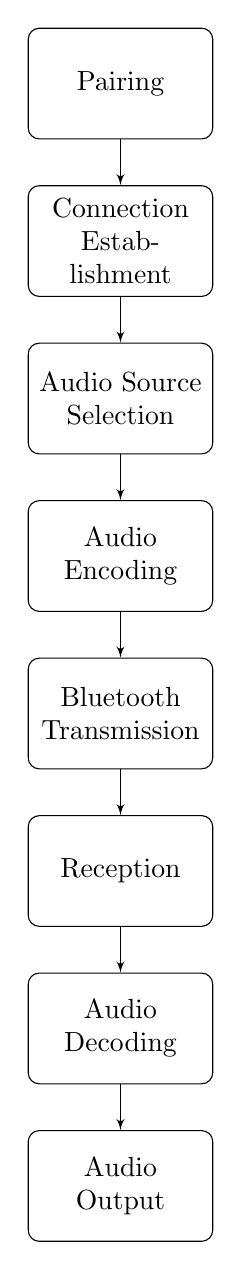
\begin{tikzpicture}[node distance = 2cm, auto]
        % Nodes
        \node [rectangle, draw, text width=6em, text centered, rounded corners, minimum height=4em] (pairing) {Pairing};
        \node [rectangle, draw, below of=pairing, text width=6em, text centered, rounded corners, minimum height=4em] (connection) {Connection Establishment};
        \node [rectangle, draw, below of=connection, text width=6em, text centered, rounded corners, minimum height=4em] (source) {Audio Source Selection};
        \node [rectangle, draw, below of=source, text width=6em, text centered, rounded corners, minimum height=4em] (encoding) {Audio Encoding};
        \node [rectangle, draw, below of=encoding, text width=6em, text centered, rounded corners, minimum height=4em] (transmission) {Bluetooth Transmission};
        \node [rectangle, draw, below of=transmission, text width=6em, text centered, rounded corners, minimum height=4em] (reception) {Reception};
        \node [rectangle, draw, below of=reception, text width=6em, text centered, rounded corners, minimum height=4em] (decoding) {Audio Decoding};
        \node [rectangle, draw, below of=decoding, text width=6em, text centered, rounded corners, minimum height=4em] (output) {Audio Output};

        % Arrows
        \path [draw, -latex'] (pairing) -- (connection);
        \path [draw, -latex'] (connection) -- (source);
        \path [draw, -latex'] (source) -- (encoding);
        \path [draw, -latex'] (encoding) -- (transmission);
        \path [draw, -latex'] (transmission) -- (reception);
        \path [draw, -latex'] (reception) -- (decoding);
        \path [draw, -latex'] (decoding) -- (output);
    \end{tikzpicture}
    \caption{Bluetooth Audio Transmission Process}
    \label{fig:bluetooth_process}
\end{figure}

Past 2010, under the supervision of SIG, Bluetooth LE was established which operates under a
similar premise compared to conventional Bluetooth, but was different in that it had
energy-saving measures to help battery-powered devices last for a long time. This is
accomplished by having the device in sleep mode for most of the time until communication was
established from the 'host' devices.\cite{bhalla_unraveling_2021} Bluetooth LE makes use its
unique data advertising for device discovery and connection, which can further be used to
advertise general application data to an unlimited number of listeners. LE is not directly
compatible with conventional bluetooth, but both implementations can be physically applied to
the hardware so it can use either one.\cite{bhalla_unraveling_2021} In regards to the radio
frequencies used, LE makes use of 40 channels that are hopped with FHSS at slower rates to
conserve power, which can enable multiple exchanges while on the same channel.
\cite{noauthor_bluetooth_nodate} This particular technology sees frequent use in wireless
audio, because specializations were made that allowed for a consistent exchange while
conserving energy and thus prolonging battery life.\cite{bhalla_unraveling_2021}

% Insert 802.11 WiFi Audio tidbit here 
Lorem ipsum dolor sit amet, consectetur adipiscing elit. Quod cum accidisset ut alter alterum
necopinato videremus, surrexit statim. Videamus igitur sententias eorum, tum ad verba
redeamus. Duo Reges: constructio interrete. Quam ob rem tandem, inquit, non satisfacit? Res
enim se praeclare habebat, et quidem in utraque parte. Quae tamen a te agetur non melior,
quam illae sunt, quas interdum optines. Earum etiam rerum, quas terra gignit, educatio
quaedam et perfectio est non dissimilis animantium. Alterum significari idem, ut si
diceretur, officia media omnia aut pleraque servantem vivere. Id enim natura desiderat.
Quamquam ab iis philosophiam et omnes ingenuas disciplinas habemus;

% Insert NFC tidbit here
Lorem ipsum dolor sit amet, consectetur adipiscing elit. Quod cum accidisset ut alter alterum
necopinato videremus, surrexit statim. Videamus igitur sententias eorum, tum ad verba
redeamus. Duo Reges: constructio interrete. Quam ob rem tandem, inquit, non satisfacit? Res
enim se praeclare habebat, et quidem in utraque parte. Quae tamen a te agetur non melior,
quam illae sunt, quas interdum optines. Earum etiam rerum, quas terra gignit, educatio
quaedam et perfectio est non dissimilis animantium. Alterum significari idem, ut si
diceretur, officia media omnia aut pleraque servantem vivere. Id enim natura desiderat.
Quamquam ab iis philosophiam et omnes ingenuas disciplinas habemus;

% Future technology and correspondence portion
In addition to the previously discussed technologies, there are emergent audio technologies
that are pushing the envelope of wireless high-fidelity (Hi-Fi) audio. One such technology
involves a proprietary wireless communication standard that is capable of transmitting audio
at a 16ms latency: The AIAIAI Audio UNIT-4 Wireless+ speakers with the W+ Link technology.
This particular technology does not have publicly available specifications, but AIAIAI have
stated some of the key differences that distinguishes it from bluetooth. One such difference
is that the W+ Link technology makes use of two antennas for reception and transmission of
information as opposed to the singular antenna that Bluetooth makes use of. What the presence
of two antennas entail is the ability to swap between one or the other if one connection
drops out. Additionally, the technology prioritizes keeping the same latency by means of
swapping between pre-defined radio frequency bands as opposed to using a pseudorandom
pattern. Additionally, the W+ Link technology does not compress audio, delivering it at a 44.
1 kHz 16-bit quality, roughly equating to a little over 1400 Kbps.\cite{noauthor_unit-4_2023}

\begin{figure}[htbp]
    \centering
    \includegraphics[width=1\linewidth]{Unit-4_wireless_showcase.jpg}
    \caption{AIAIAI UNIT-4 Wireless+ \cite{noauthor_unit-4_2023}}
    \label{fig:unit-4_productPic}
\end{figure}

\section*{Conclusion and Future Work}

To be added...

\bibliographystyle{IEEEtran}
\bibliography{cmpe189}

\vspace{12pt}
\end{document}
